\documentclass[a4paper,12pt,french]{article}

\usepackage[utf8]{inputenc}
\usepackage[T1]{fontenc}
\usepackage[upright]{kpfonts}

\usepackage{amsmath,amsfonts,amssymb}
\usepackage[margin=1.4cm]{geometry}
\usepackage{enumitem}
\usepackage[lastexercise]{exercise}
\usepackage{multicol}
\usepackage{tikz}
\usepackage{tkz-tab}
\usetikzlibrary{babel}
\usepackage{babel}

\setlength{\columnseprule}{0pt}

%\setlength{\parindent}{0pt}
\setlist{noitemsep}
%\setlist[1]{\labelindent=\parindent} % < Usually a good idea
\setlist[itemize]{leftmargin=*}
\setlist[itemize,1]{label=$\blacktriangleright$}
\setlist[enumerate]{labelsep=*, leftmargin=1.5pc}
\setlist[enumerate,1]{label=\arabic*., ref=\arabic*}
\setlist[enumerate,2]{label=\emph{\alph*}),
ref=\theenumi.\emph{\alph*}}
\setlist[enumerate,3]{label=\roman*), ref=\theenumii.\roman*}
\setlist[description]{font=\sffamily\bfseries}

\renewcommand{\ExerciseName}{Exercice}
\renewcommand{\AnswerName}{Réponse de l'exercice}

\newcommand{\abs}[1]{\left\lvert #1\right\rvert}

\newcommand{\N}{\mathbf{N}}
\newcommand{\R}{\mathbf{R}}

\everymath{\displaystyle\everymath{}}

\title{Méthode de Héron}
\date{20 octobre 2015}

\begin{document}

\maketitle

\begin{Exercise}[number=104]
  L'activité 3 nous a permis d'introduire la notion de limite d'une
  suite et de faire la conjecture

  $f$ est la fonction définie sur $\R^*$ par : \[ f(x) = \frac12\left(x
  + \frac2x\right).\]

  \begin{enumerate}
    \item \begin{enumerate}
        \item Justifier que $f$ est dérivable pour tout $x$ de $\R^*$.
        \item Démontrer que pour tout $x$ de $\R^*$ : \[ f'x) = \frac{
          (x - \sqrt{2})(x + \sqrt{2})}{2x^2}.\] Déduisez-en le tableau
          de variation de $f$ sur $\R^*$.
      \end{enumerate}
    \item La suite $(u_n)_{n\in\N}$ est définie par $u_0 = \frac32$ et
      pour tout entier naturel $n$, $u_{n+1} = f(u_n)$.
      \begin{enumerate}
        \item Calculez $u_1$ et $u_2$. (Donnez les résultats sous la
          forme de fractions, puis sous forme décimale arrondie à
          $10^{-5}$.)
        \item Démontrez par récurrence que pour tout entier naturel $n$,
          $\sqrt{2} < u_{n+1} < u_n \leqslant \frac32$.

          Déduisez-en que la suite $(u_n)_{n\in\N}$ est convergente.
        \item Démontrez que pour tout $n$ de $\N$, \[ u_{n+1} - \sqrt{2}
          < \frac12\left(u_n - \sqrt{2} \right).\]
        \item Déduisez-en par récurrence que tout tout $n$ de $\N$, \[ 0
            < u_n - \sqrt{2} \leqslant \frac1{2^n}\left(u_0 - \sqrt{2}
          \right). \]
        \item Déduisez-en $\lim_{n\to+\infty}u_n$.
      \end{enumerate}
  \end{enumerate}
\end{Exercise}
\begin{Answer}[number=104]
  \begin{enumerate}
    \item \begin{enumerate}
        \item $f$ est la somme (à un coefficient multiplicatif près) de
          deux fonctions dérivables, l'une pour tout $x$ de $\R^*$
          seulement, donc elle est dérivable.
        \item Démontrons que pour tout $x$ de $\R^*$ : \[ f'x) = \frac{
          (x - \sqrt{2})(x + \sqrt{2})}{2x^2}.\] 

          D'une part, $f'(x) = \frac12\left( 1 - \frac2{x^2}\right) =
          \frac{x^2 -2}{2x^2}$ par le calcul direct de la dérivée.

          D'autre part, $(x-\sqrt{2})(x+\sqrt{2}) = x^2 - 2$.

          On a donc l'égalité demandée.

          $\forall x\in\R^*,\ 2x^2 > 0$ le signe de la dérivée est le
          signe du numérateur. On en déduit le tableau de variation
          ci-dessous :

          \begin{center}
            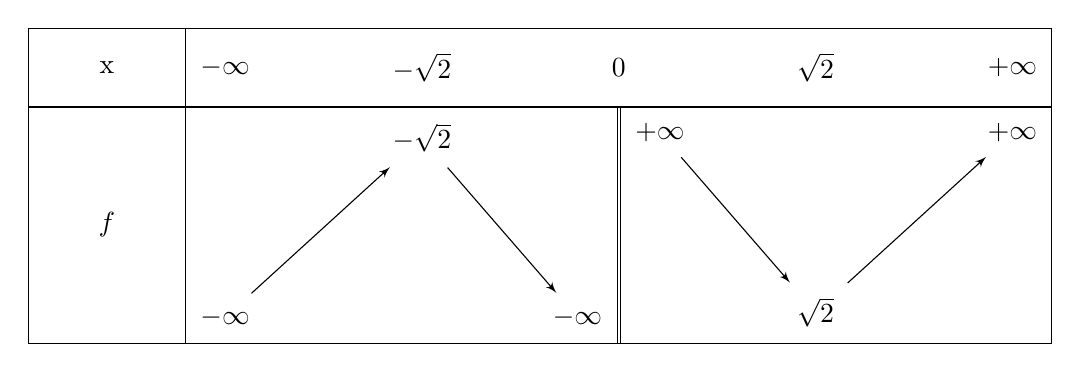
\begin{tikzpicture}
              \tkzTabInit[espcl=2.5]
              {   x / 1 , $f$ /3 }%
              {$-\infty$ , $-\sqrt2$    , 0  ,  $\sqrt2$, $+\infty$ }%
              \tkzTabVar{ -/$-\infty$ , +/$-\sqrt2$ , -D+/$-\infty$/$+\infty$,
              -/$\sqrt2$, +/$+\infty$ }
            \end{tikzpicture}
          \end{center}

      \end{enumerate}
    \item La suite $(u_n)_{n\in\N}$ est définie par $u_0 = \frac32$ et
      pour tout entier naturel $n$, $u_{n+1} = f(u_n)$.
      \begin{enumerate}
        \item $u_1 = \frac{17}{12} \approx 1,41666$ et $u_2 =
          \frac{577}{408} \approx 1,41421$.
        \item Démontrons par récurrence que pour tout entier naturel $n$,
          $\sqrt{2} < u_{n+1} < u_n \leqslant \frac32$.
          \begin{itemize}
            \item Initialisation : cf calcul et comparaison de 2 et
              $u_1^2$
            \item Soit $n$ un entier naturel, supposons que $P_n$ : «
              $\sqrt{2} < u_{n+1} < u_n \leqslant \frac32$ » soit vraie
              et démontrons $P_{n+1}$ : «$\sqrt{2} < u_{n+2} < u_{n+1}
              \leqslant \frac32$ ».

              $f$ est croissante sur $[\sqrt{2} ; 4]$, $P_n \implies
              f(\sqrt{2}) < f(u_{n+1}) < f(u_n) \leqslant
              f\left(\frac32\right)$.

              $f(\sqrt{2}) = \sqrt{2}\ ;\ f(u_{n+1}) = u_{n+2}\ ;\
              f(u_n) = u_{n+1}\ ;\ f\left(\frac32\right) \leqslant 32$

              On a donc $P_{n+1}$.
            \item En utilisant le principe de récurrence, on a la
              conclusion : $\forall n\in\N,\ \sqrt{2} < u_{n+1} < u_n
              \leqslant \frac32$
          \end{itemize}

          La suite $(u_n)_{n\in\N}$ est décroissante, minorée donc
          convergente.
        \item Démontrons que pour tout $n$ de $\N$, \[ u_{n+1} - \sqrt{2}
          < \frac12\left(u_n - \sqrt{2} \right).\]
          Soit $n$ un entier naturel,

          $u_{n+1} - \sqrt{2} = \frac12\left(u_n - \frac2{u_n} \right) -
          \sqrt{2} = \frac12\left(u_n - \frac{2\sqrt{2}}{u_n}\right)$

          $u_n -\frac{2\sqrt2}{u_n} < u_n - \sqrt2 \iff 0< 2\sqrt{2} -
          u_n\sqrt2 \iff u_n < 2$, qui est réalisé, voir question
          précédente.
        \item Formalisons par récurrence que tout tout $n$ de $\N$, \[ 0
            < u_n - \sqrt{2} \leqslant \frac1{2^n}\left(u_0 - \sqrt{2}
          \right). \]
          \begin{itemize}
            \item C'est $u_0 \leqslant u_0$ donc vraie au rang 0.
            \item Supposons vrai au rang $n$, alors

              $u_{n+1} - \sqrt{2} < \frac12 \left(u_n - \sqrt{2}\right)
              \leqslant \frac12 \frac1{2^n}\left(u_0 - \sqrt{2} \right)
              = \frac1{2^{n+1}}\left(u_0 - \sqrt{2} \right)$
            \item Conclusion : $\forall n\in\N,\ u_n - \sqrt{2}
              \leqslant \frac1{2^n}\left(u_0 - \sqrt{2} \right)$.
          \end{itemize}
          Pour l'autre partie de l'inégalité, elle découle de 2.b)
        \item Pour tout $n$ entier naturel, la suite définie par $u_n -
          \sqrt2$ est encadrée par la suitee nulle et une suite
          géométrique de raison positive inférieure strictement à 1.
          Cette suite est donc de limite nulle.

          Il vient que $\lim_{n\to+\infty}u_n = \sqrt2$.
      \end{enumerate}
  \end{enumerate}
\end{Answer}
\end{document}
